\section{User Manual}
\subsection{Registration and Login}
An unregistered \textbf{User} can have access to the service only via prior Registration.\\

\begin{figure}[H]
	\centering
	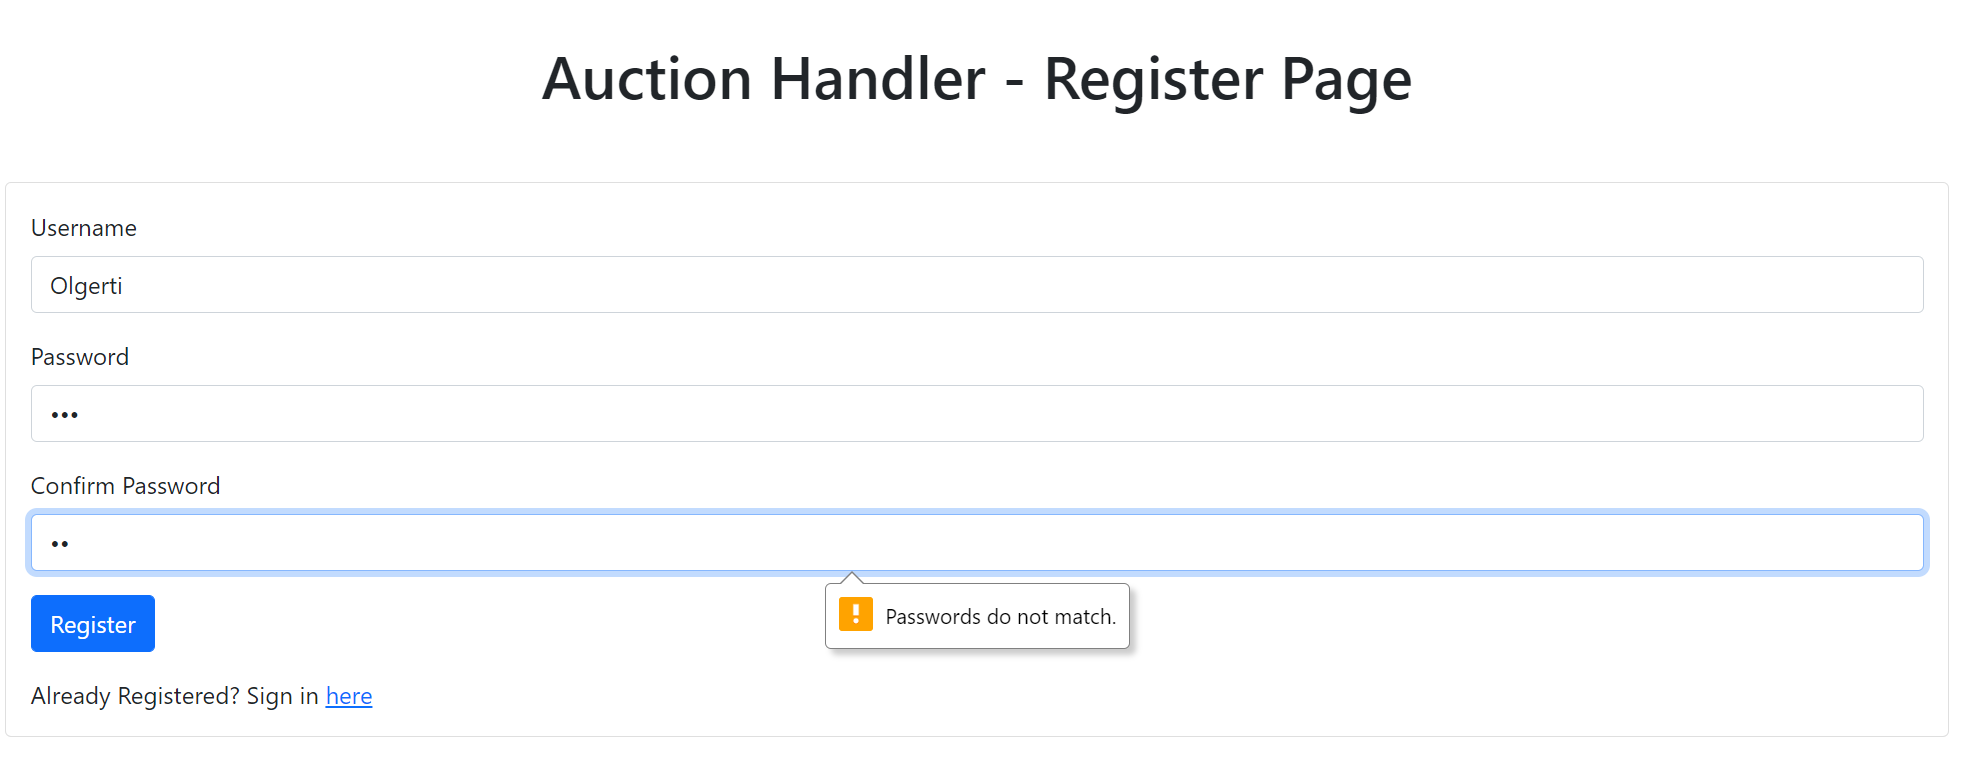
\includegraphics[width=\textwidth]{img/registration}
	\caption{Registration Page}
	\label{fig:registration}
\end{figure}

The registration page only involves the insertion of \textit{username} and \textit{password} fields. If the two passwords do not match a pop-up will be show to the \textbf{User}, as shown in the above figure.\\

\noindent After a successful registration, the \textbf{User} needs to login to the service, this can be done via a dedicated page to do so as shown in the figure below.

\begin{figure}[H]
	\centering
	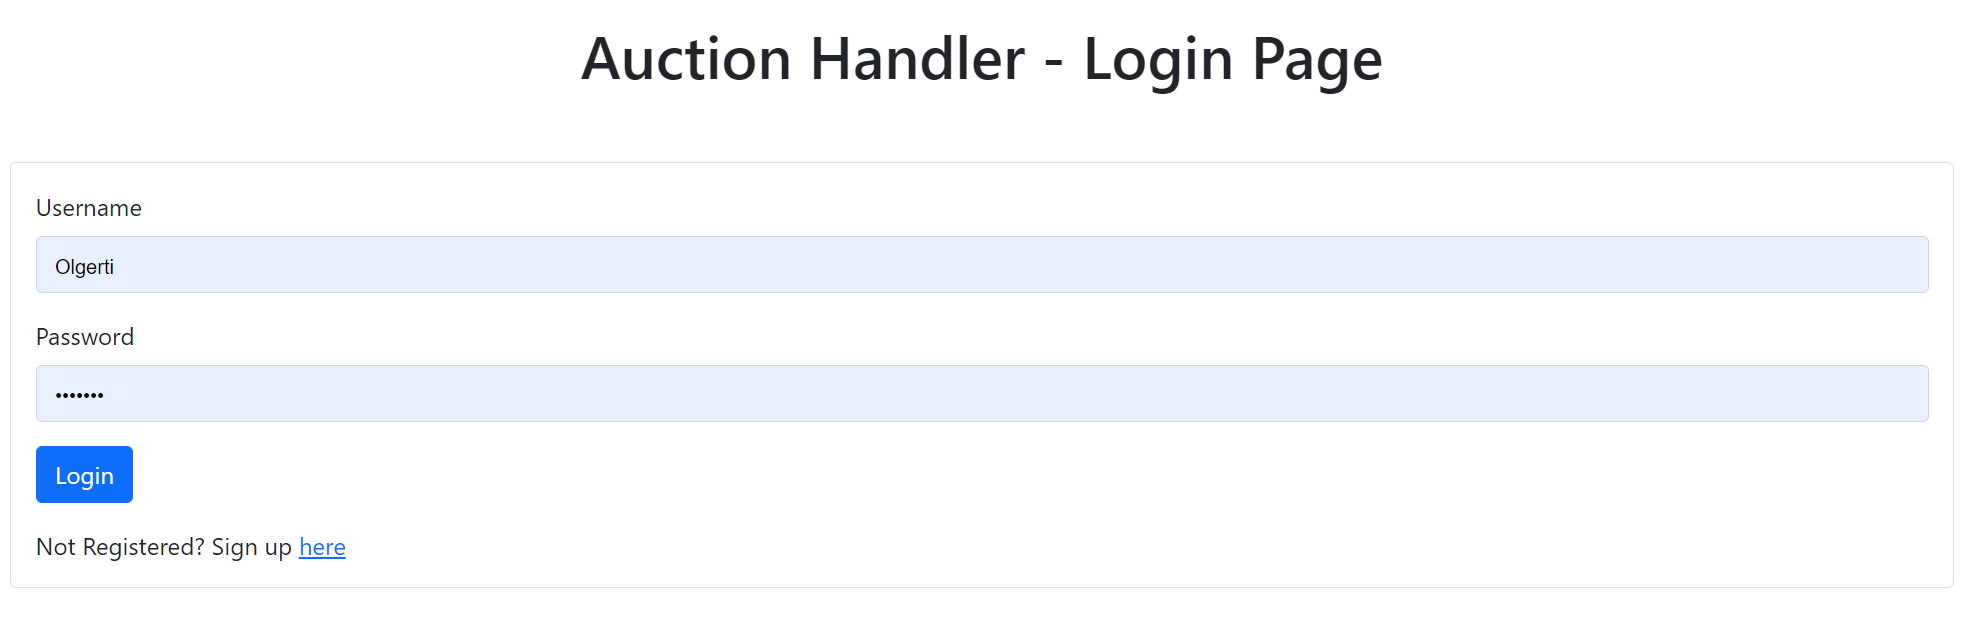
\includegraphics[width=\textwidth]{img/login}
	\caption{}
	\label{fig:login}
\end{figure}

\subsection{Main Menu and Auction Creation}
A logged \textbf{User} has the possibility to see an overview of the ongoing auctions and the results of past auctions (in terms of who was the winner). For the latter in no winner was elected (i.e. due to lack of bids), the winner will be called \textit{NoWinner}.
\begin{figure}[H]
	\centering
	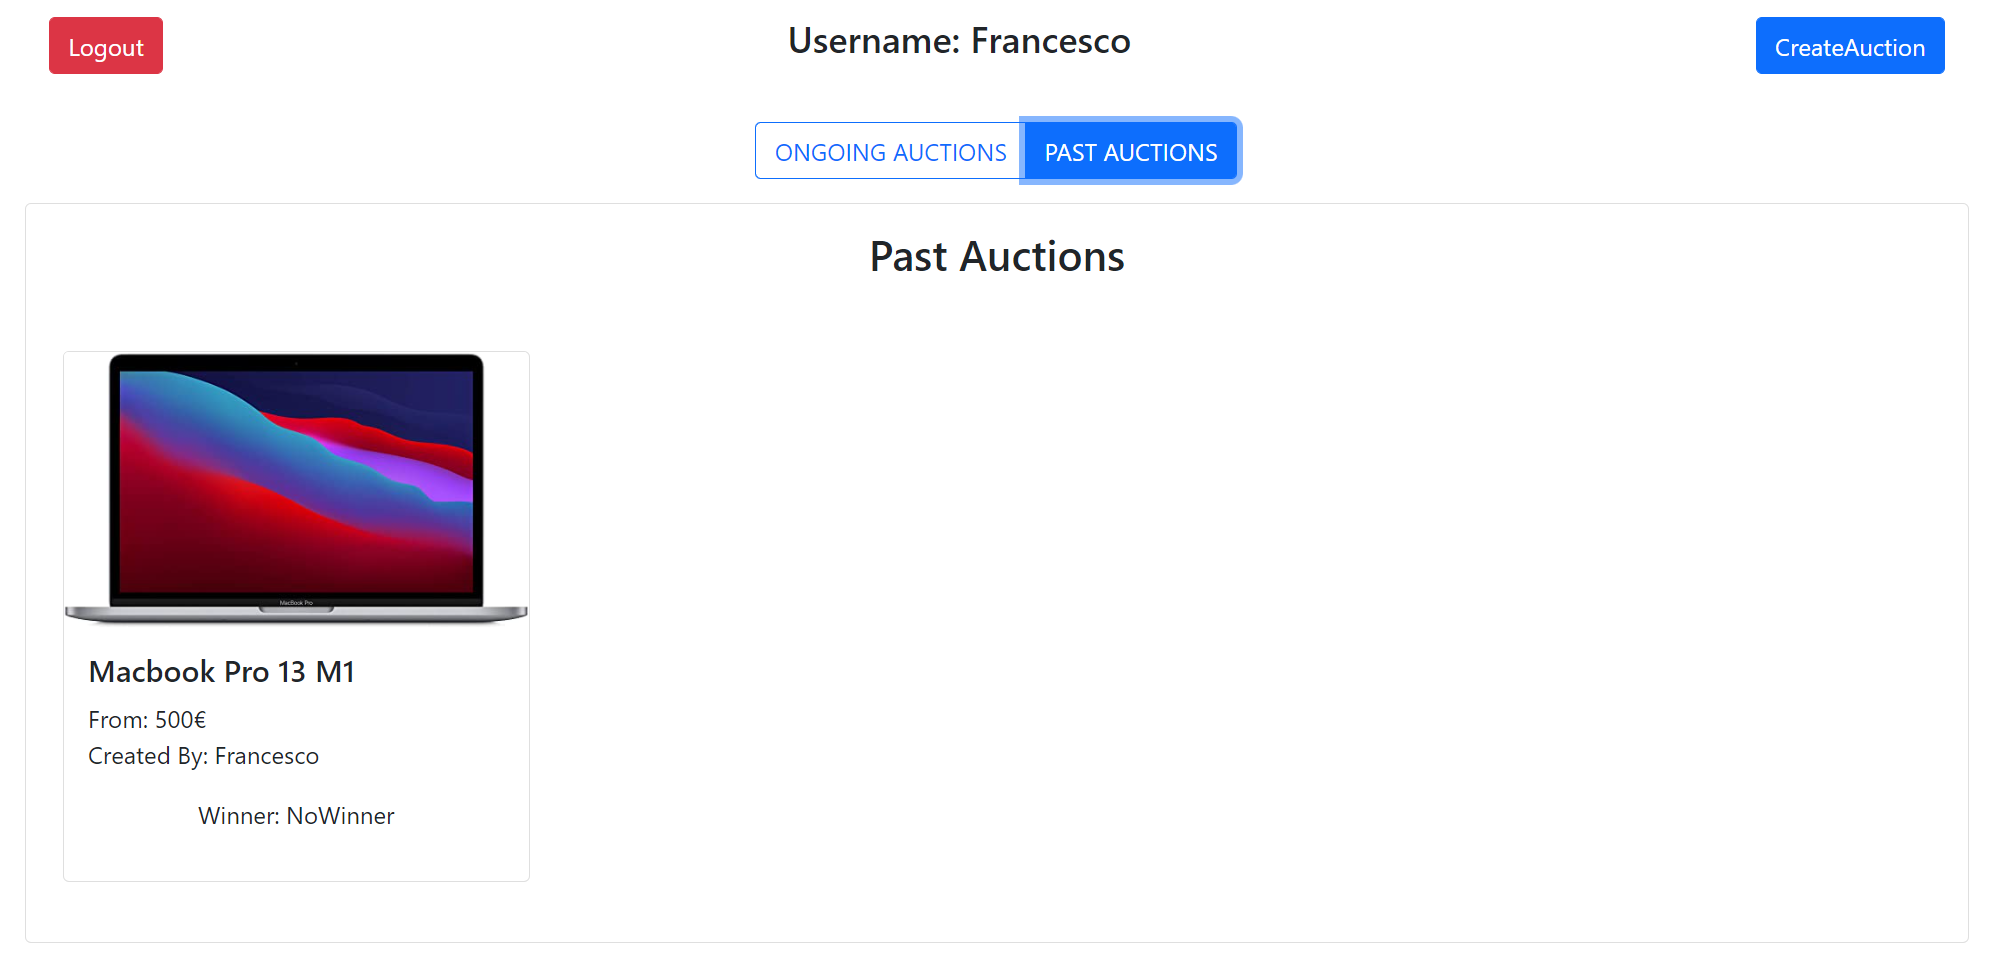
\includegraphics[width=\linewidth]{img/past_auctions}
	\caption{Past Auctions Tab}
	\label{fig:pastauctions}
\end{figure}

A \textbf{User} can also participate to an ongoing auction by pressing the related button of the ongoing auctions tab. 

\begin{figure}[H]
	\centering
	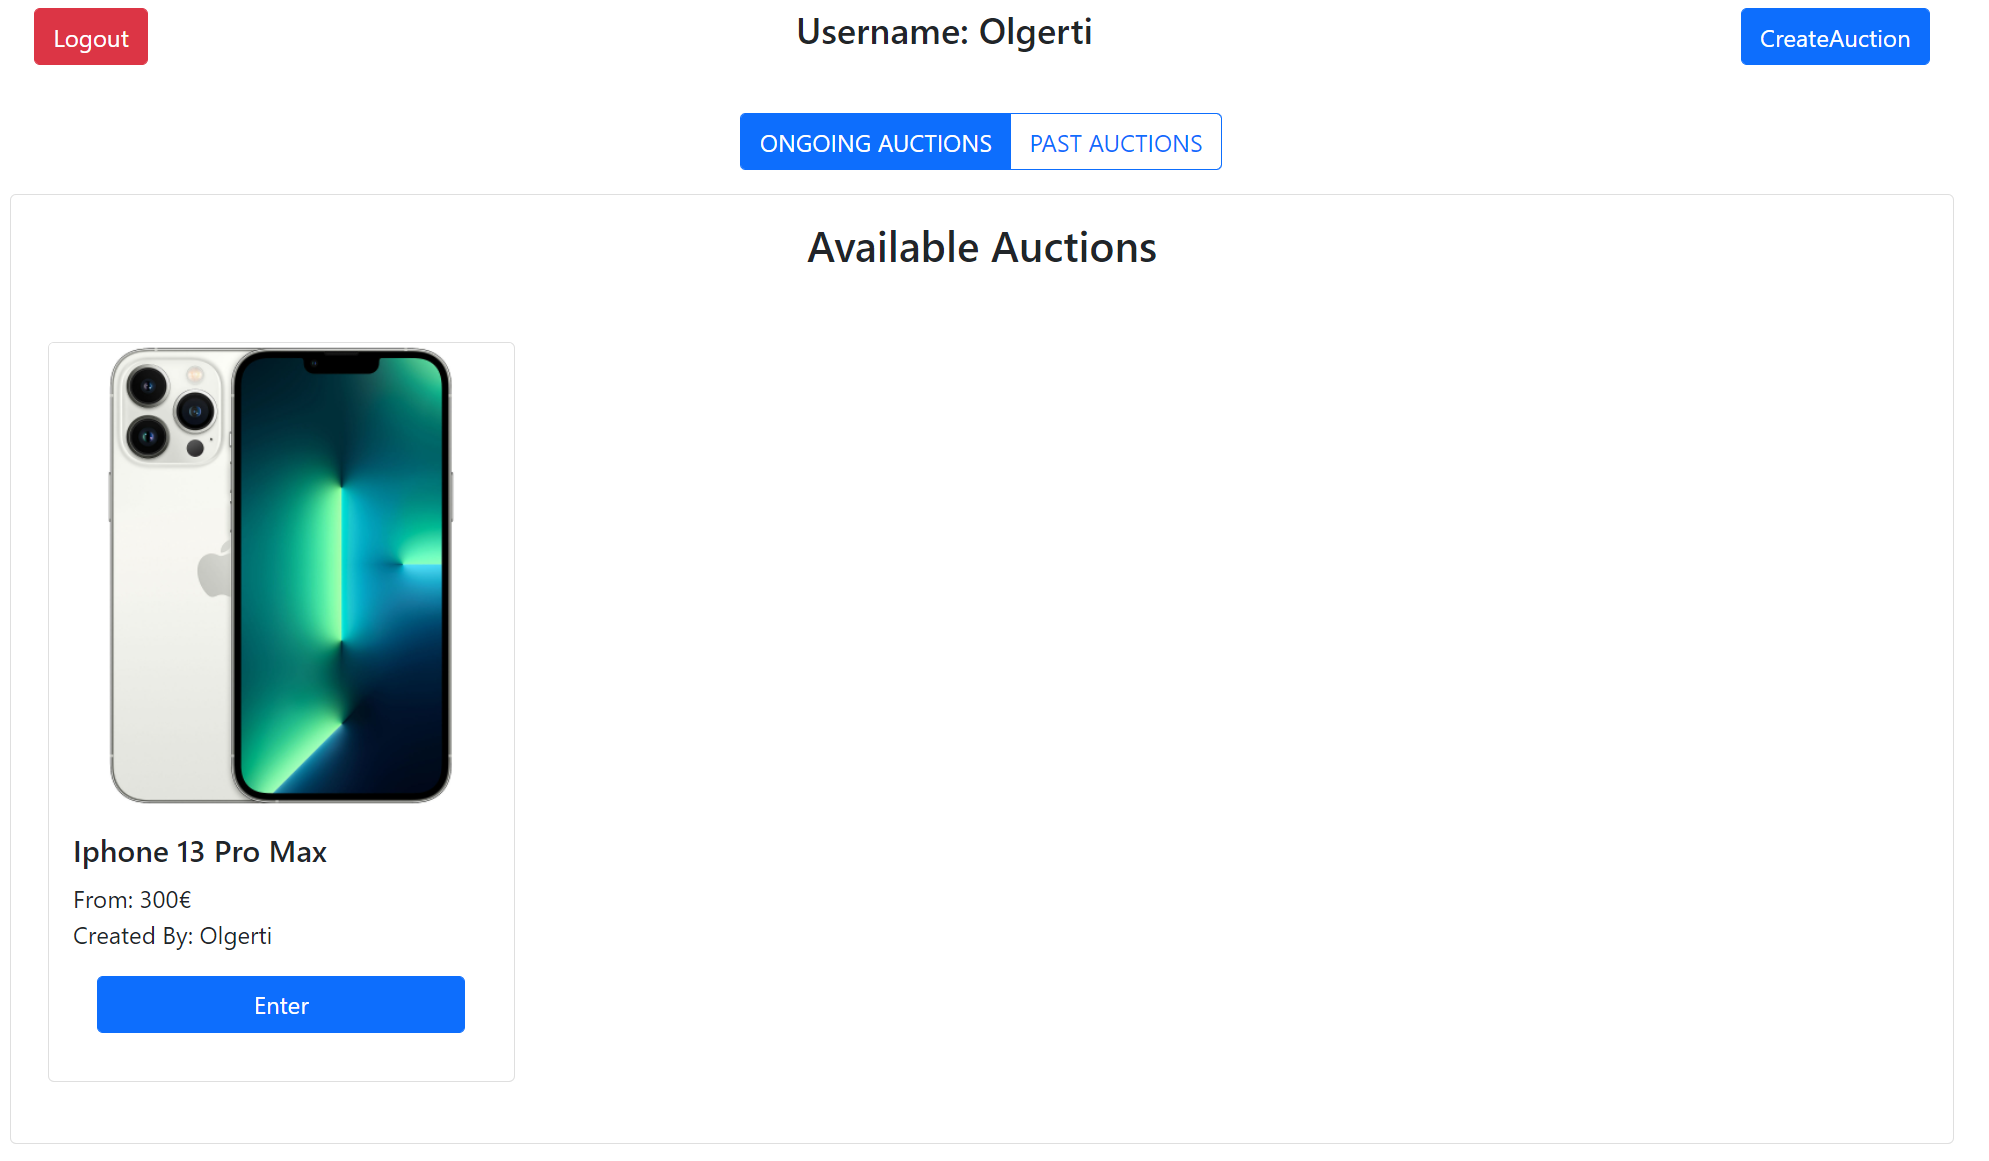
\includegraphics[width=1\linewidth]{img/active_auctions}
	\caption{Active Auctions Tab}
	\label{fig:activeauctions}
\end{figure}


A \textbf{User} has also the possibility to create his own auction by pressing the \textit{CreateAuction} button in the Main Menu. Another form will be shown as can be seen in the figure below.

\begin{figure}[H]
	\centering
	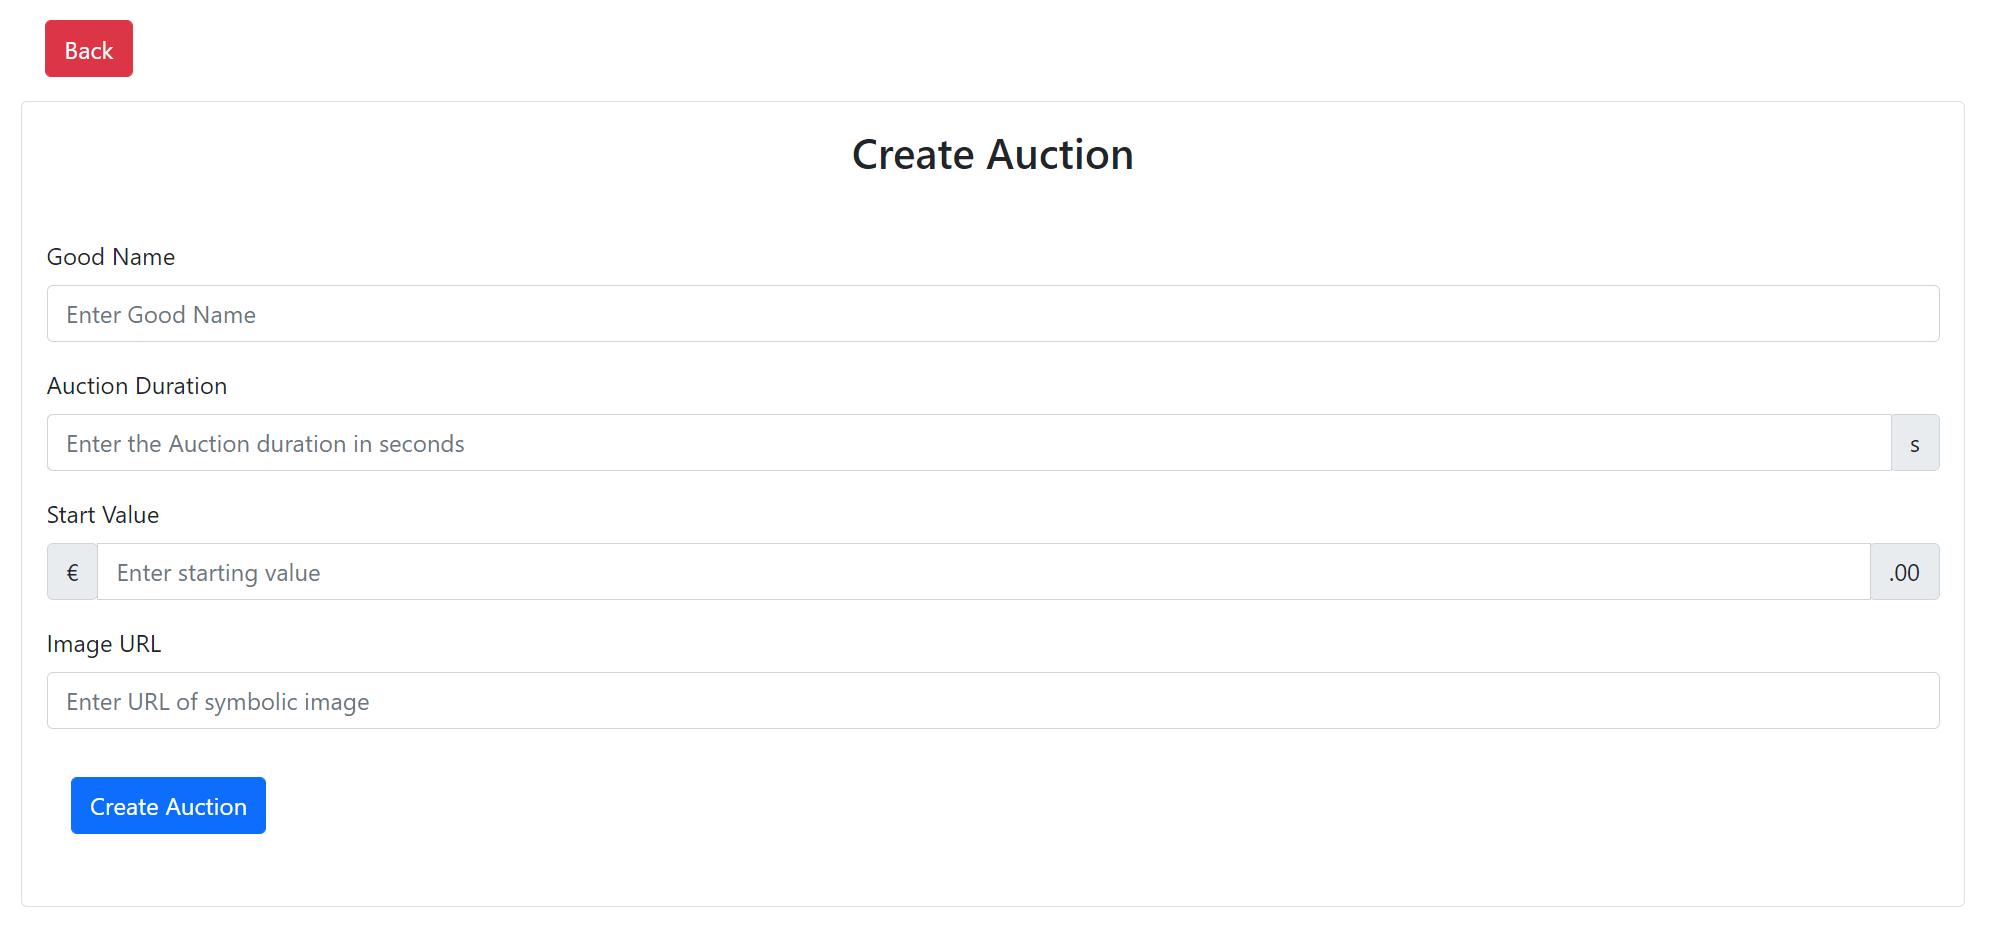
\includegraphics[width=1\linewidth]{img/create_auction}
	\caption{Create Auction Page}
	\label{fig:createauction}
\end{figure}

The \textbf{User} needs to add information about the \textit{auction duration}, the \textit{minimum bid} for the auction, the \textit{good name} to sell (which must be unique) and an \textit{image URL}. If the URL is invalid a default placeholder will be shown.

A logged \textbf{User} can perform logout by pressing the \textit{Logout} button in the Main Menu.

\subsection{Auction and Winner Election}

When an auction is created or when a \textbf{User} joins an ongoing auction, the following page will be shown:

\begin{figure}[H]
	\centering
	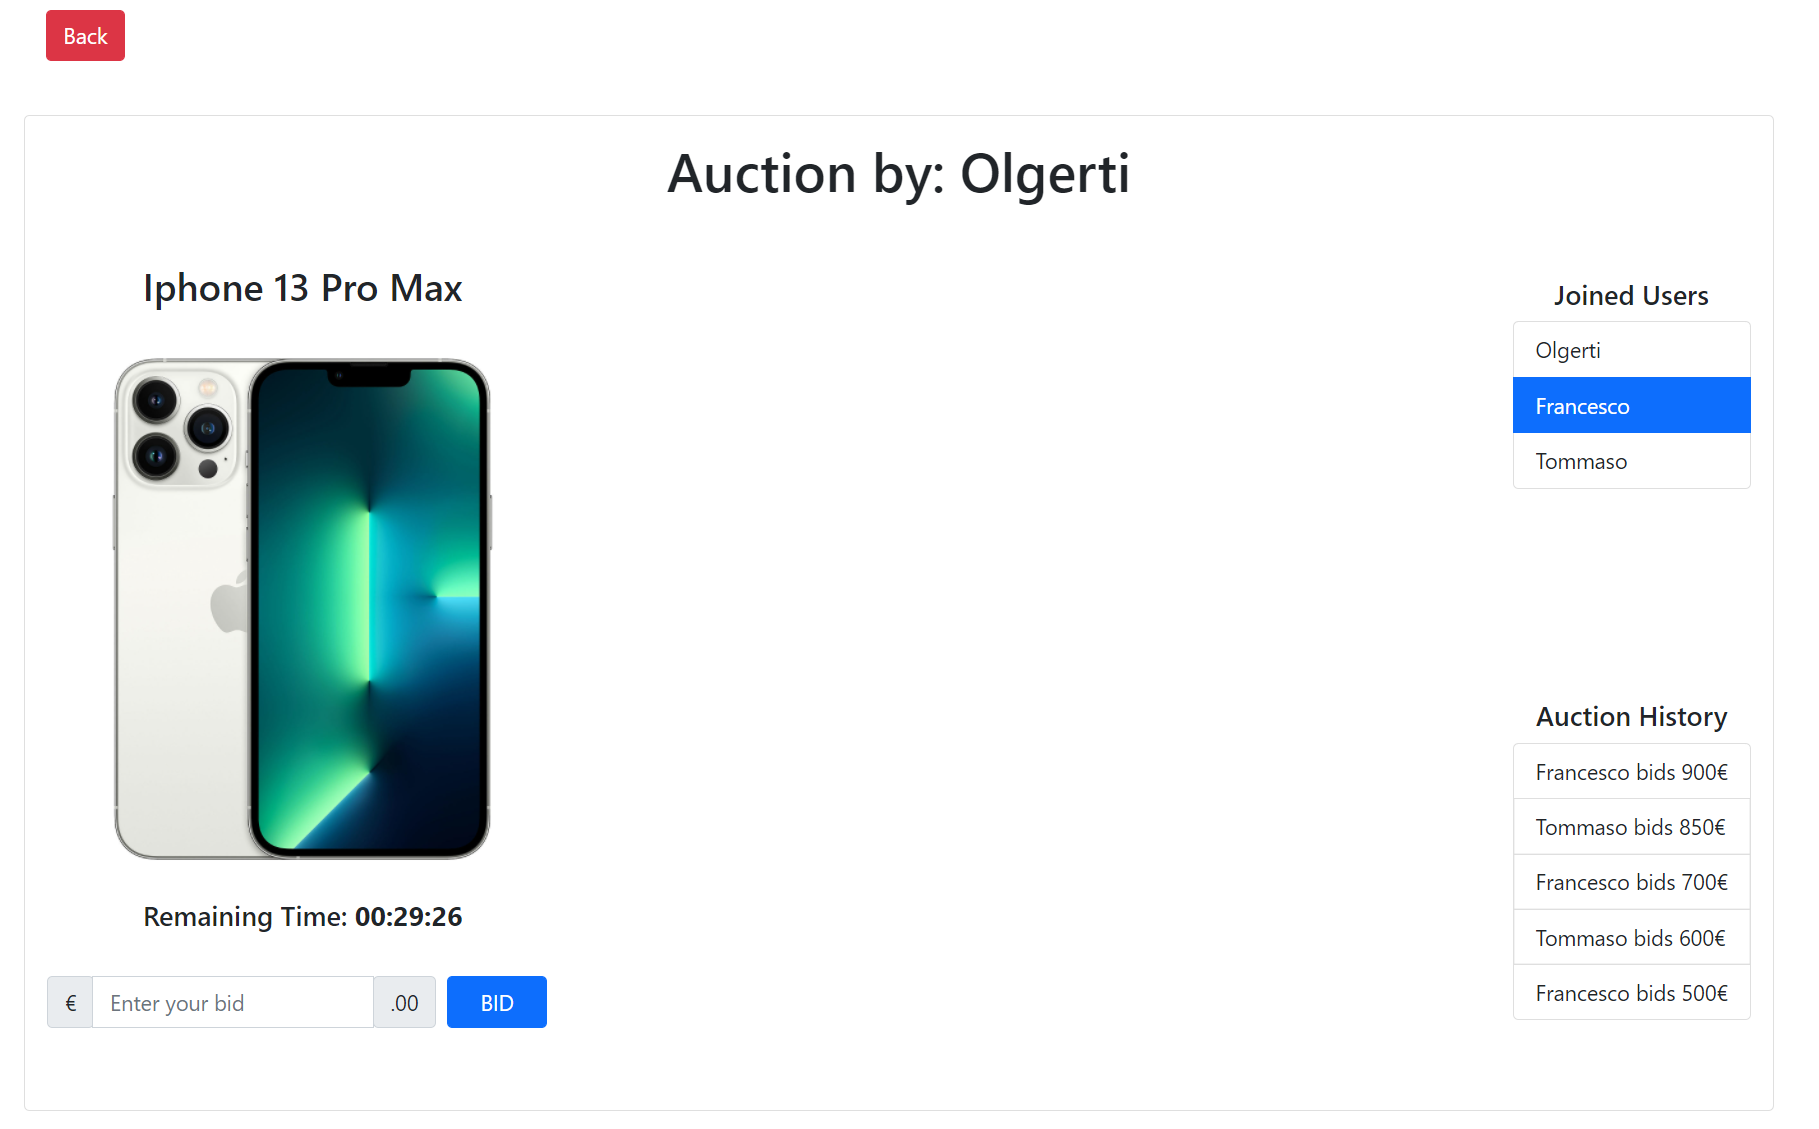
\includegraphics[width=1\linewidth]{img/auction}
	\caption{}
	\label{fig:auction}
\end{figure}

On the upper-right corner is shown the list of joined users. On the bottom-right corner the current list of valid bids that were made. A \textbf{User} can send a bid for the good if and only if it is not the creator of the auction and the bid value is higher than the last accepted bid (the first one shown in the Auction History table). If no bid are present then the bid value must be higher than the \textit{minimum bid} inserted at auction creation.
A \textbf{User} can decide to exit from the auction by pressing the \textit{Back} button.
At the end of the auction, each connected user will see the auction result by means of a pop-up, as shown in the figure below.

\begin{figure}[H]
	\centering
	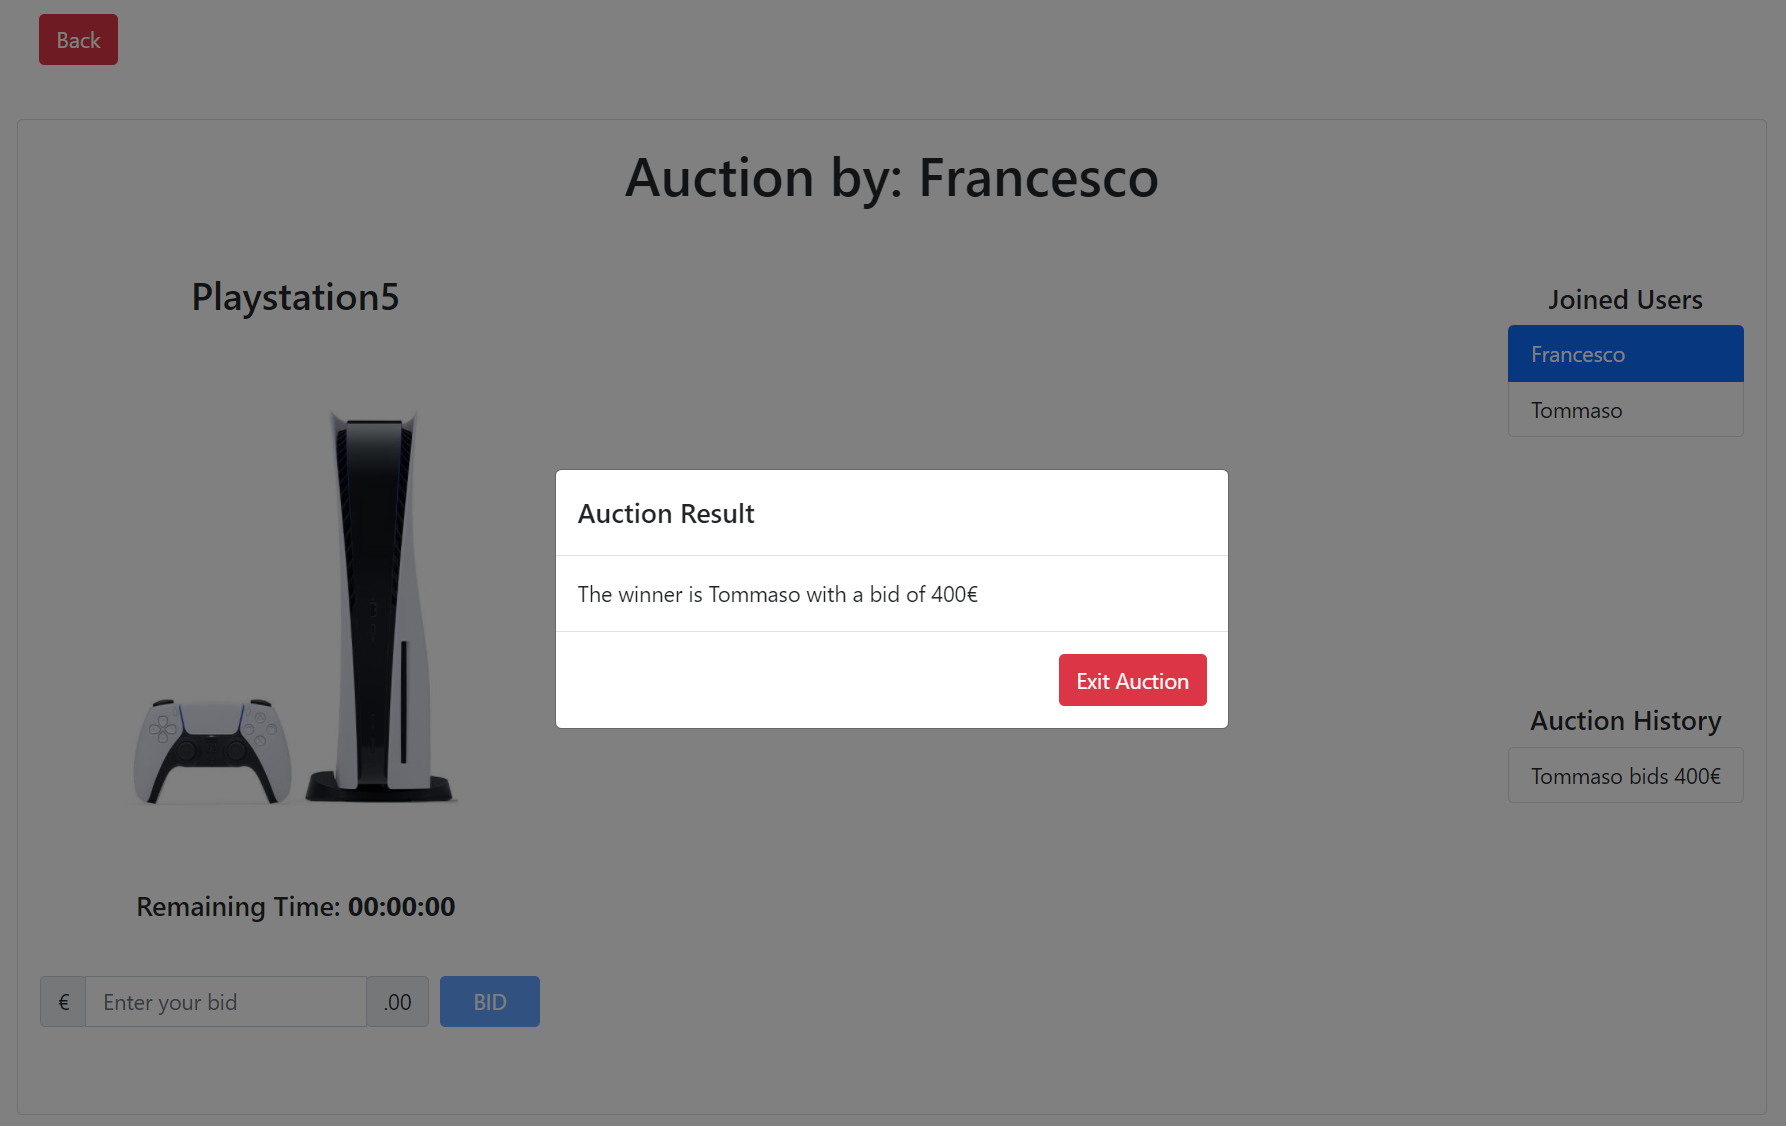
\includegraphics[width=1\linewidth]{img/auction_finish}
	\caption{Auction Results}
	\label{fig:auctionfinish}
\end{figure}
